\documentclass[crop=false, class=book]{standalone}

\usepackage{lipsum}

\begin{document}
	\chapter{Introduzione}
	
	Il sequenziamento del DNA costituisce una tecnica fondamentale per lo studio del genoma di una specie, perché permette di determinare l'ordine delle basi azotate dei nucleotidi che costituiscono il DNA. Tale processo trova applicazione in molti studi biologici che riguardano vari ambiti, come ad esempio la medicina riproduttiva, l'oncologia o l'infettivologia, attraverso indagini tra cellule diverse dello stesso individuo o lo studio delle mutazioni genetiche tra individui di una stessa specie \cite{shendure2012expanding}. 
	
	% CONTENUTI (ordine da determinare)
	% a cosa serve (es: Assembly)
	% breve storia 
	% metodi (sperimentali vs computazionali) -> k-mer
	% cosa sono i k-mer
	
	\section{Storia}
	Lo studio approfondito del DNA si sviluppa a partire dal 1953, con la scoperta della sua struttura tridimensionale ad opera di James Watson e Francis Crick \cite{watson1953molecular}, contribuendo all'analisi dell'azione degli acidi nucleici nella sintesi proteica. Solo nel 1977 però, vennero sviluppate le prime strategie sperimentali per il sequenziamento, come il famoso metodo Sanger \cite{sanger1977DNA, sanger1977nucleotide} TODO
	
	
	\section{Sequenze di lunghezza k: i k-mer}
		TODO
		
	\subsection{K-mer profile}
	\label{subsec:kmerprofile}
	Il \textit{k-mer profile}, detto anche \textit{k-mer spectrum}, conta la frequenza dei k-mer trovati nelle letture di input, non assemblate o allineate. Esso può rappresentare un indicatore della complessità del genoma preso in esame \cite{vurture2017genomescope}, e mostra la quantità di k-mer distinti trovati ad una certa frequenza. Un esempio di k-mer profile è mostrato dalla figura~\vref{fig:profilecomp} tratta da \cite{sohn2016present}, in cui si può notare come la natura del genoma influenzi direttamente il grafico. 

	
	\begin{figure}
		\centering
		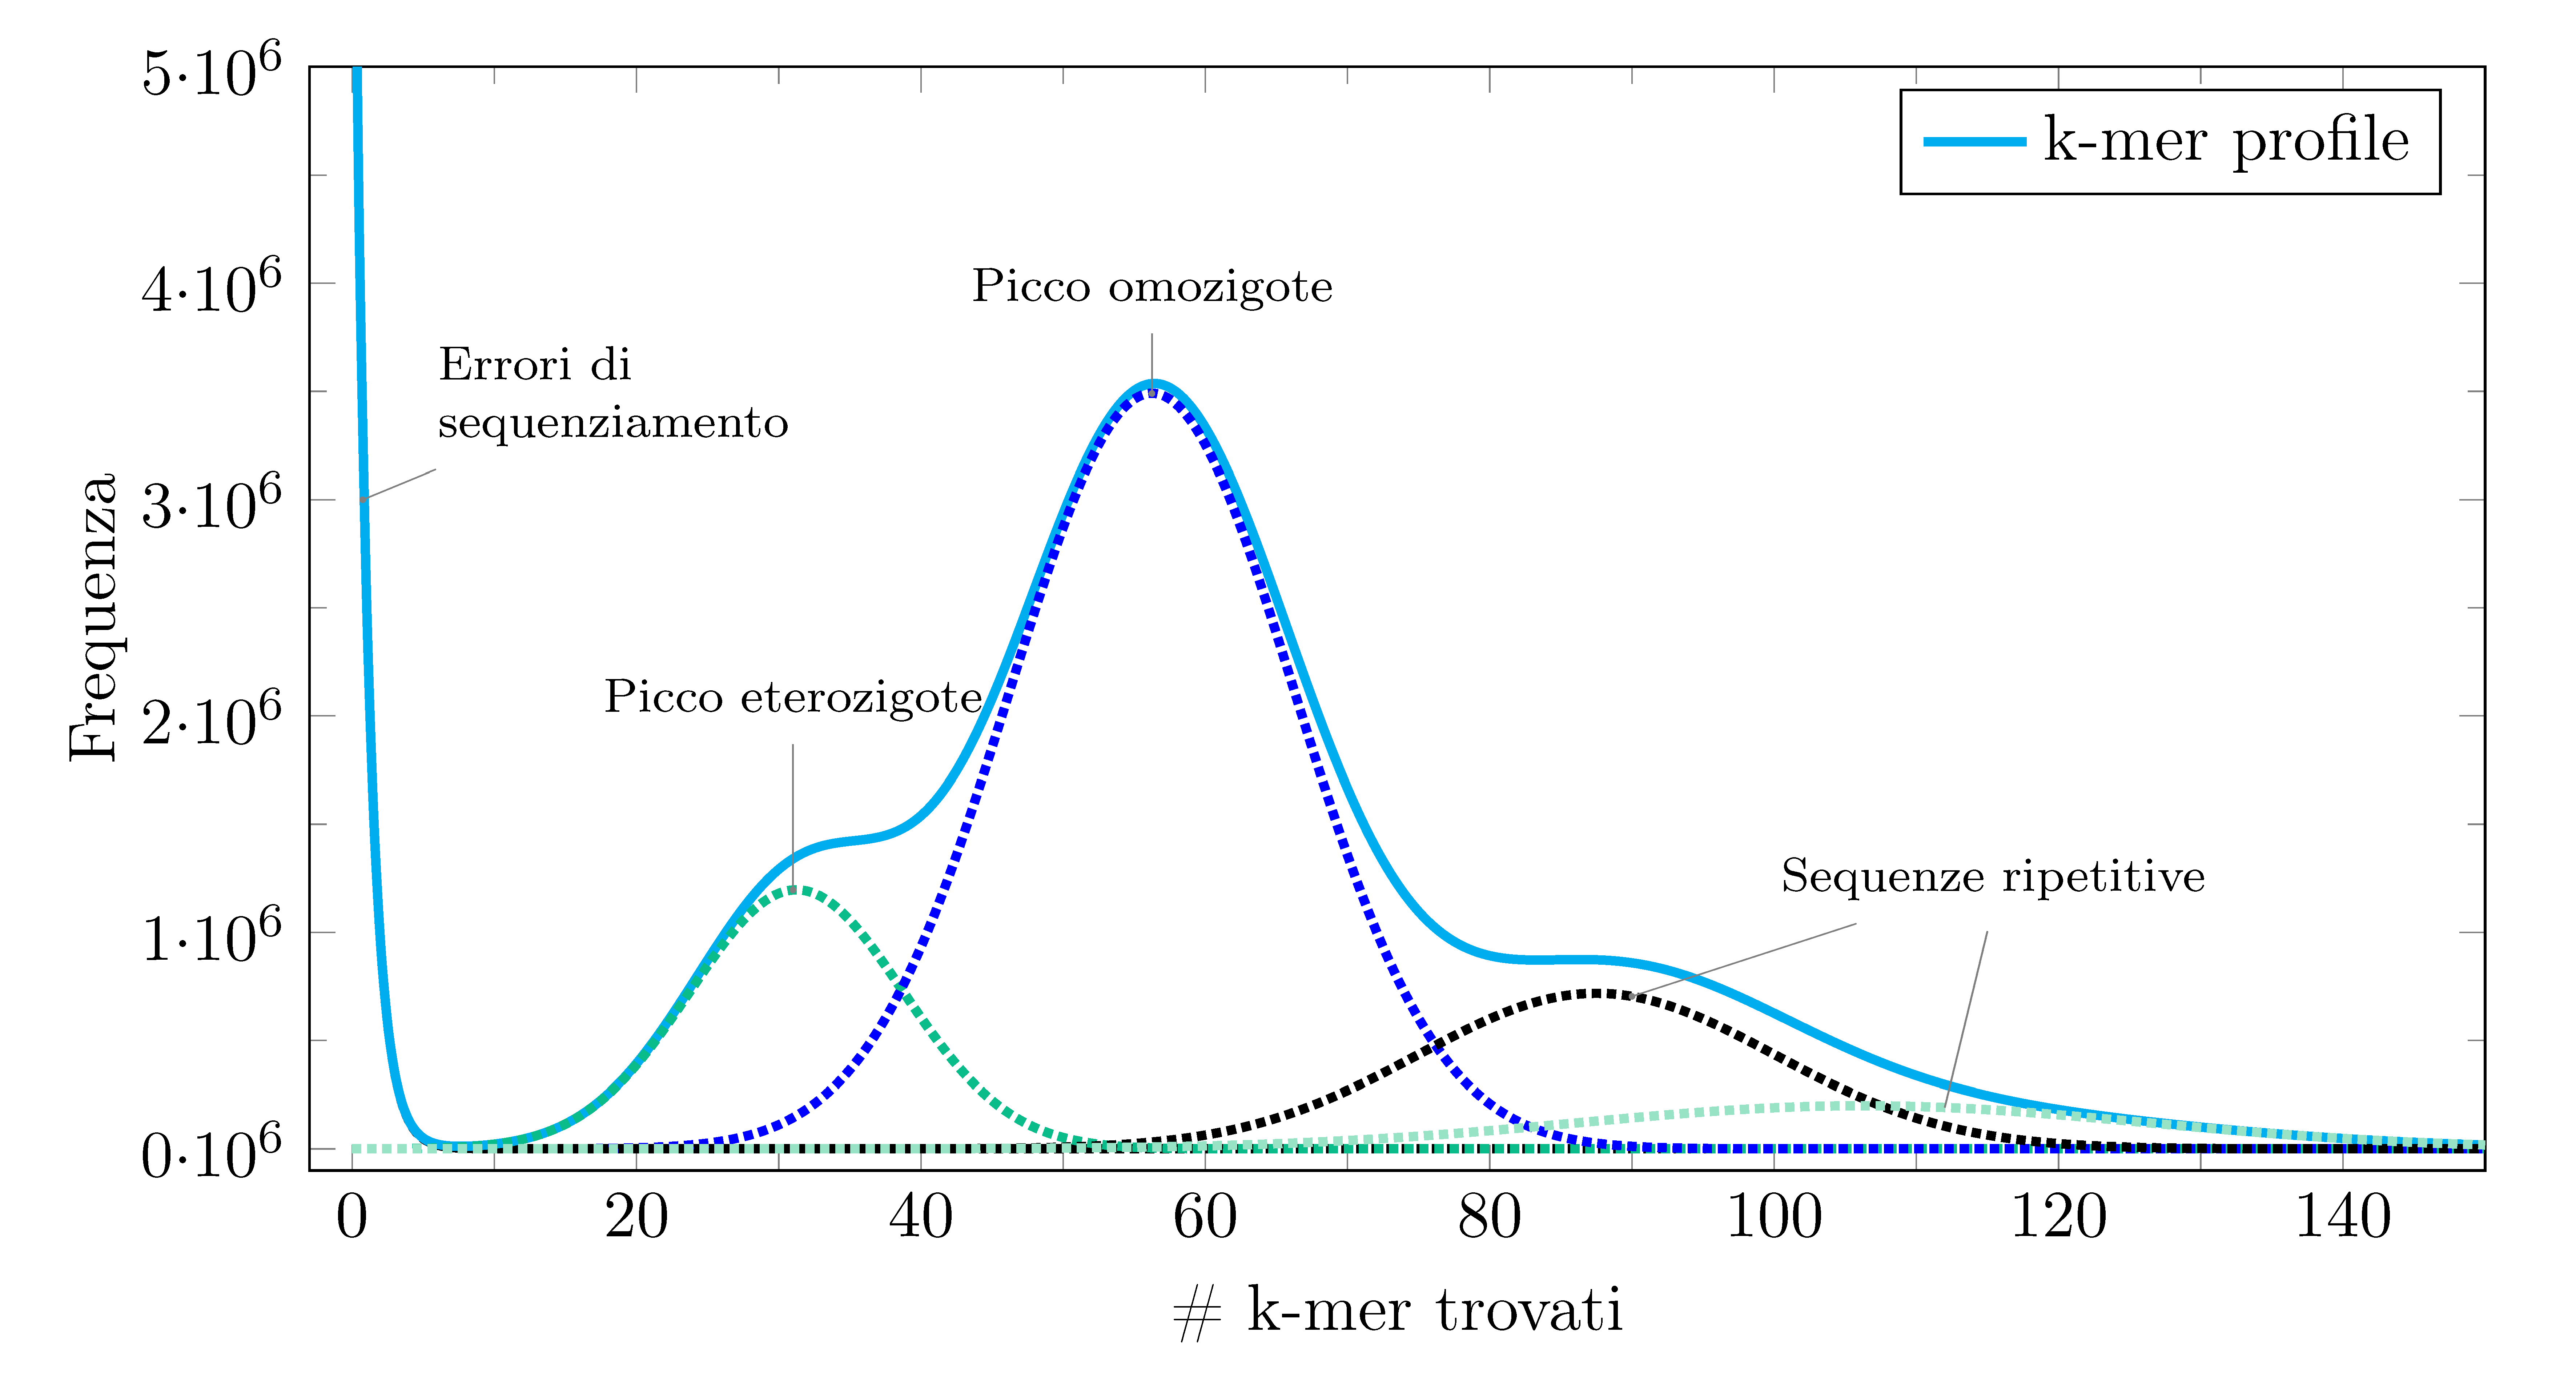
\includegraphics[width=0.8\textwidth]{capitoli/introduzione/profilecomp.png}
		\caption{TODO.}
		\label{fig:profilecomp}
	\end{figure}
	
	Ipotizzando che il genoma sia ideale, omozigote e senza ripetizioni, e che le letture siano state fatte senza errori con una certa copertura, il grafico del k-mer profile sarà una \gls{dp} centrata sulla copertura media disponibile.
	
	In casi reali invece, il genoma sarà eterozigote con una certa percentuale di eterozigosi e saranno presenti errori di sequenziamento; il k-mer profile presenterà tre picchi principali~\cite{sun2017findGSE}.
	Il primo picco del grafico corrisponde ai k-mer derivati da errori di sequenziamento, che accadono spesso ma che hanno bassa frequenza perché presentano poche occorrenze nelle letture di input; il secondo invece, rappresenta i k-mer eterozigoti e il terzo quelli omozigoti, presenti quindi su uno o entrambi gli alleli del set di cromosomi. I k-mer eterozigoti devono essere trattati più attentamente, perché possono risultare simili a quelli del primo picco, derivanti da errori di sequenziamento~\cite{sohn2016present}.	
	
	La lunga coda della distribuzione rappresenta invece le sequenze ripetitive, che occorrono con alta frequenza e sono presenti in un elevato numero di \gls{locus}. Eventuali ripetizioni aggiungono al grafico ulteriori picchi, mentre errori nelle letture aumentano la varianza e producono distorsioni nel grafico.
	
	La figura~\vref{fig:kmerprofile} mostra come all'aumentare del \gls{rate_eterozigosity} la quantità di k-mer eterozigoti del secondo picco diventi dominante rispetto ai k-mer omozigoti del terzo picco, che invece diminuiscono.
	
	Il k-mer profile può essere calcolato tramite programmi specifici date delle letture del genoma di input, quali \textit{Jellyfish}~\cite{marcais2011fast} o \textit{KMC2}~\cite{deorowicz2015KMC}.
	
	
	
	
	\begin{figure}
		\centering
		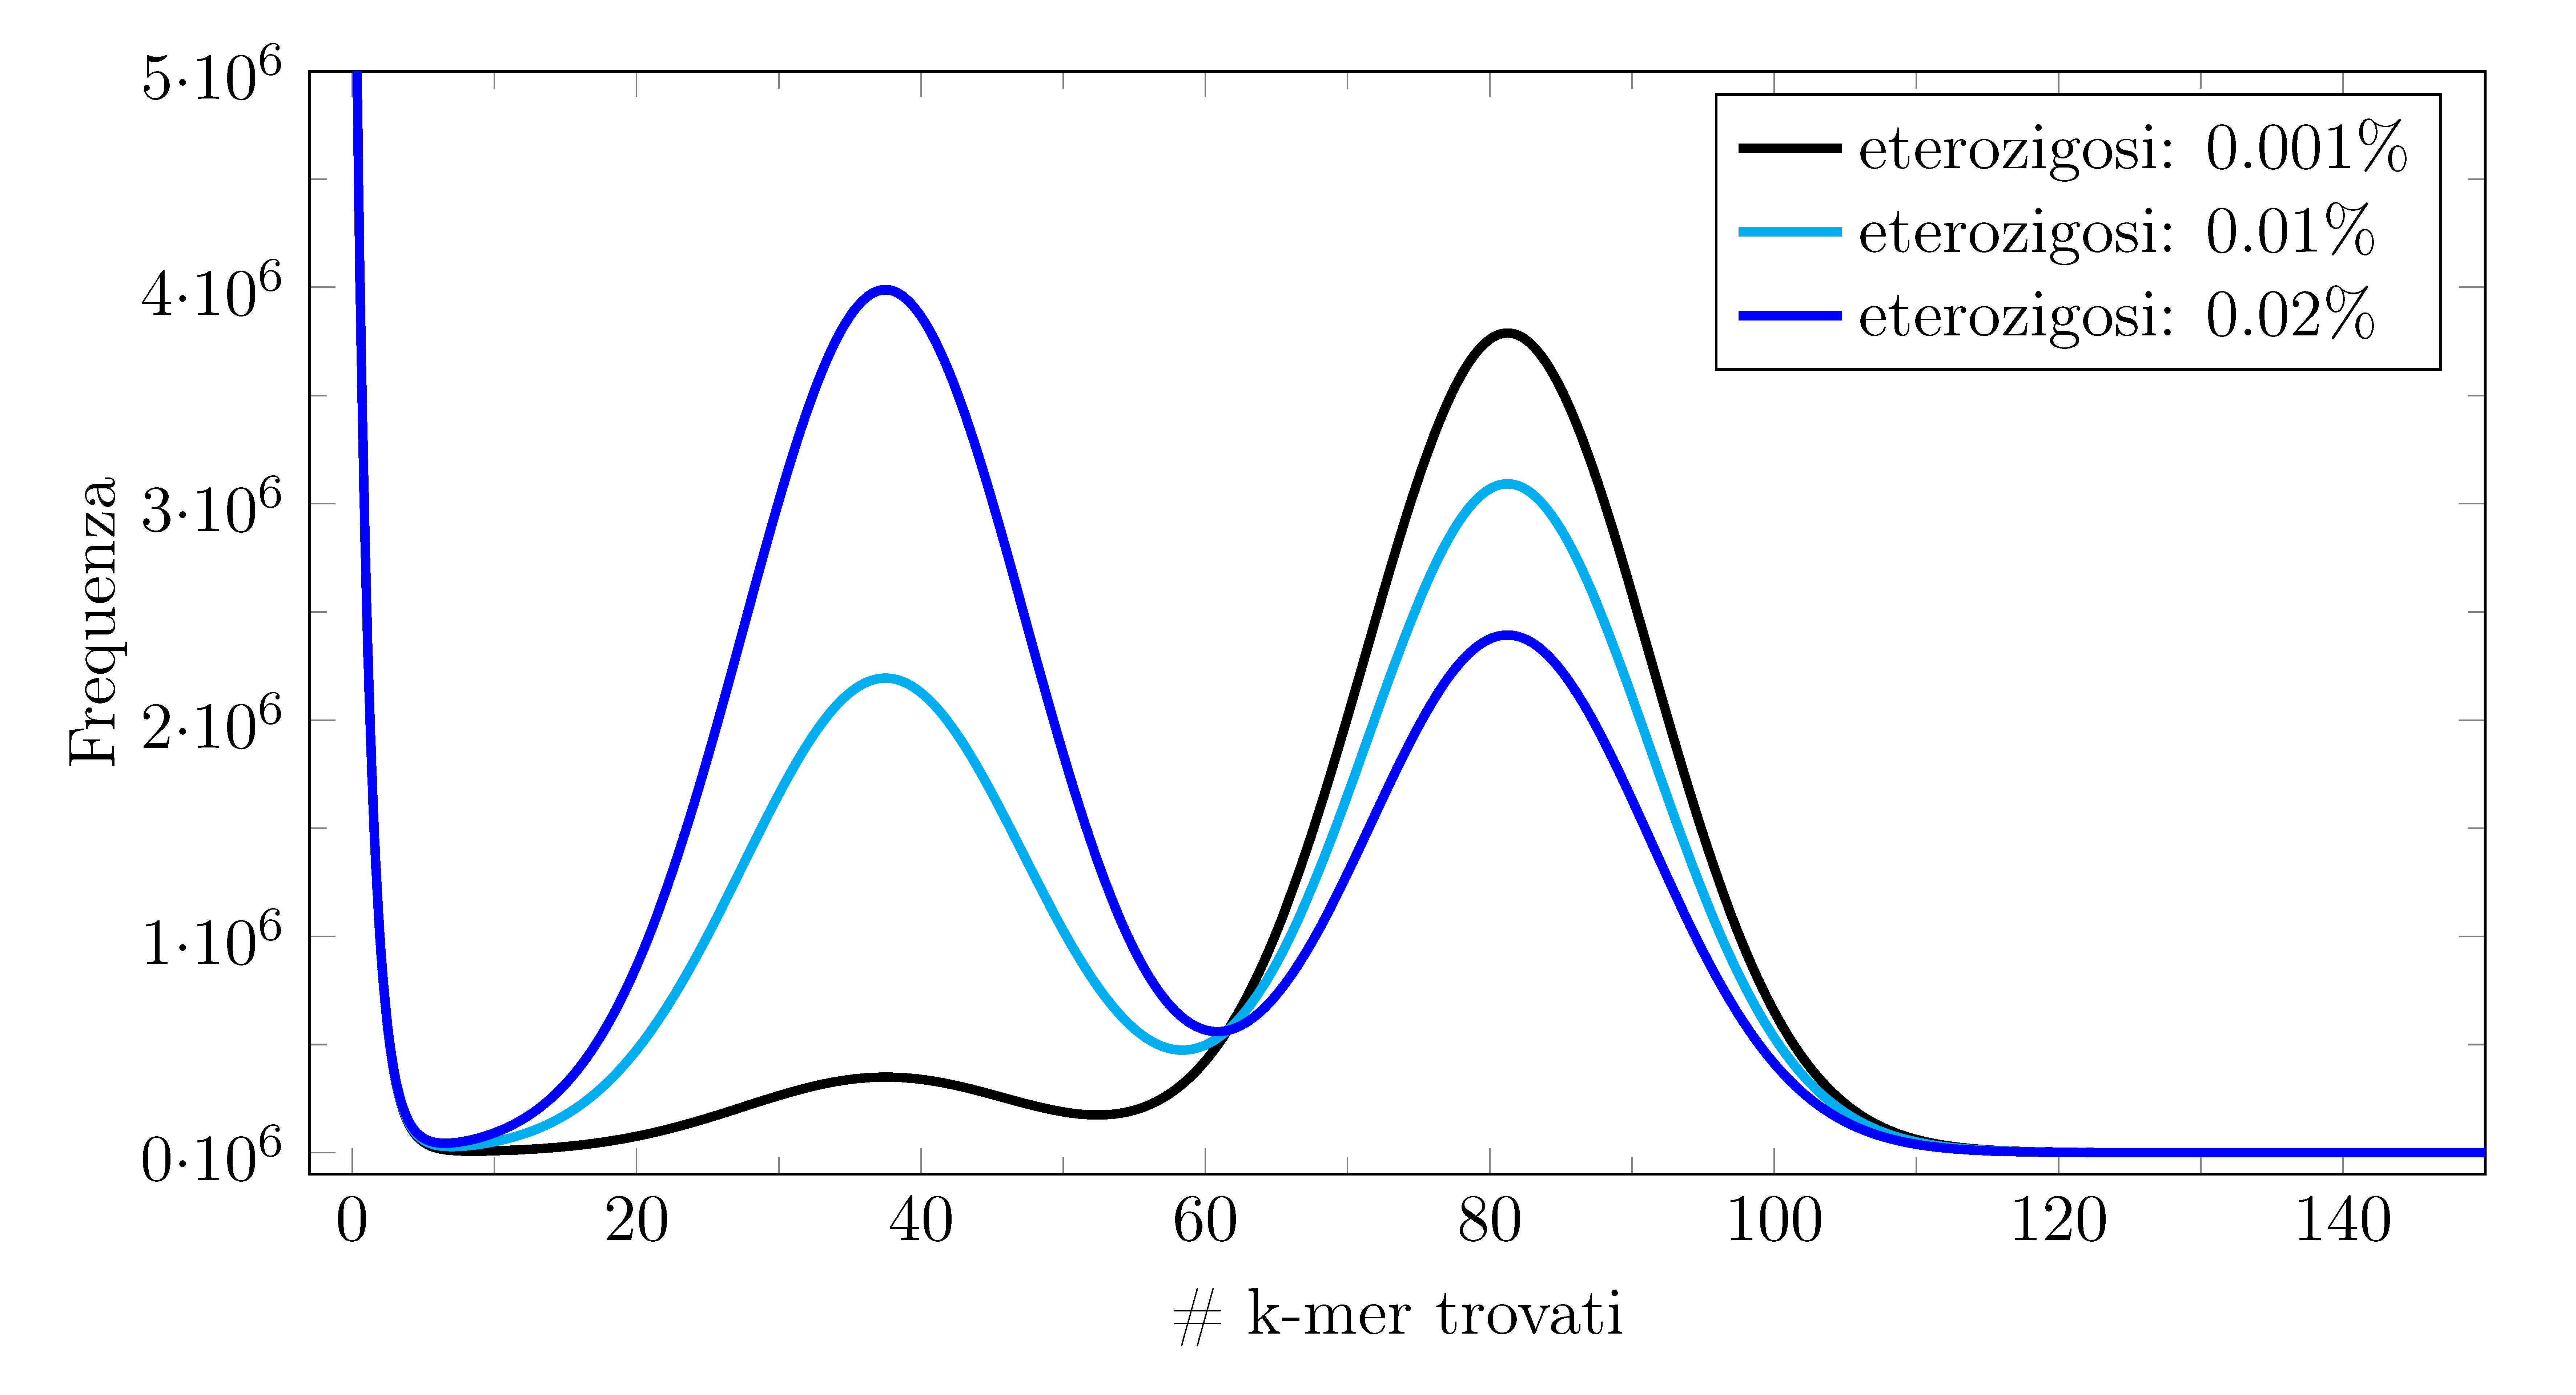
\includegraphics[width=0.8\textwidth]{capitoli/introduzione/kmerprofile.png}
		\caption{TODO.}
		\label{fig:kmerprofile}
	\end{figure}

	%\lipsum[1]
	%\section{Lorem ipsum}
	%\lipsum[2]
	%\subsection{Dolor sit amet} 
	%\lipsum[3]
	%\subsubsection{Lorem ipsum}
	%\lipsum[3]
	
	
	
	
\end{document}